\begin{figure}[H]
\centering
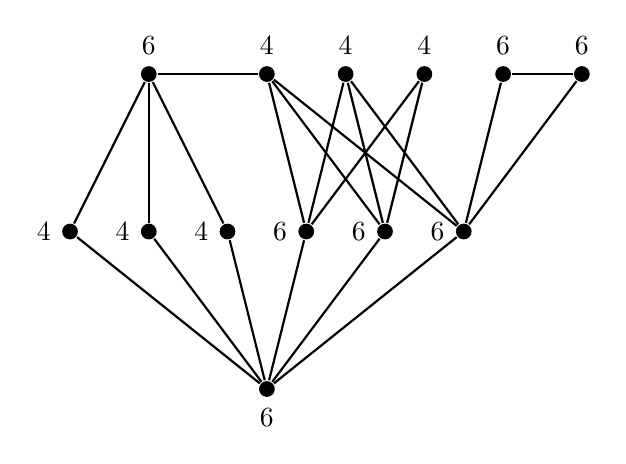
\begin{tikzpicture}[
       thick,
       acteur/.style={
         circle,
         fill=black,
         thick,
         inner sep=2pt,
         minimum size=0.2cm
       }
     ]

       \node (v) at (-3.5,0) [acteur,label=below:$6$]{};
       \node (w1) at (-6,2) [acteur,label=left:$4$]{}; 
       \node (w2) at (-5,2) [acteur,label=left:$4$]{}; 
       \node (w3) at (-4,2) [acteur,label=left:$4$]{};
       \node (w4) at (-3,2) [acteur,label=left:$6$]{};
       \node (w5) at (-2,2) [acteur,label=left:$6$]{};
       \node (w6) at (-1,2) [acteur,label=left:$6$]{};
       
       \node (u1) at (-3.5,4) [acteur,label=above:$4$]{};
  	   \node (u2) at (-2.5,4) [acteur,label=above:$4$]{};
  	   \node (u3) at (-1.5,4) [acteur,label=above:$4$]{};

	   \node (u4) at (-0.5,4) [acteur,label=above:$6$]{};
	   \node (u5) at (0.5,4) [acteur,label=above:$6$]{};
	   
  	   \node (vs) at (-5,4) [acteur,label=above:$6$]{};
  	   
       \draw (v) -- (w1);
       \draw (v) -- (w2);
       \draw (v) -- (w3);
       \draw (v) -- (w4);
       \draw (v) -- (w5);
       \draw (v) -- (w6);
       
       \draw (w4) -- (u1);
       \draw (w4) -- (u2);
       \draw (w4) -- (u3);
       \draw (w5) -- (u1);
       \draw (w5) -- (u2);
       \draw (w5) -- (u3);
       \draw (w6) -- (u1);
       \draw (w6) -- (u2);
       \draw (w6) -- (u4);
       \draw (w6) -- (u5);
       
       \draw (w1) -- (vs);
       \draw (w2) -- (vs);
       \draw (w3) -- (vs);
       
	   \draw (vs) -- (u1);
	   
	   \draw (u4) -- (u5);

\end{tikzpicture}
  \caption{The case $f=6$, $t(G)=1$}
  \label{figure12:Figure 12}
\end{figure}
